\section{Aplicación de la metodología Methadis}
Para el desarrollo del presente proyecto se aplicó la metodología Methadis de forma parcial, puesto que esta es una guía que ayuda al diseño de una aplicación hipermedia adaptativo basado en estilos cognitivos y estilos de aprendizaje. Se toman algunos elementos de esta metodología, porque el propósito de este proyecto es una aplicación hipermedia adaptativo basado solo en los estilos cognitivos. Significando esto que actividades relacionadas con los estilos de aprendizajes fueron omitidas, realizándose sólo las actividades correspondientes a los estilos cognitivos. A continuación, se muestra el proceso de aplicación de esta metodología:

\subsection{Fase I: Definición de la unidad de aprendizaje }
A raíz de los resultados arrojados por la encuesta Encuesta conocimientos previos I (véase tabla \ref{tab:CP}) se determinó que lo más conveniente, dadas las dificultades de aprendizaje de los estudiantes, era que la aplicación contará con 6 unidades de aprendizaje.

\textbf{Dominio de aprendizaje: } En cuanto al dominio del aprendizaje para cada unidad se definió que fuese de ámbito cognitivo, ya que se desea que el estudiante pueda comprender y conocer lo referente a cada una de las unidades.

\textbf{Selección de taxonomía de aprendizaje:}
En lo que se refiere a la selección de la taxonomía de aprendizaje, Methadis, señala que esta debe establecerse para facilitar la definición de los objetivos de aprendizaje, los cuales se buscó que el estudiante logre al finalizar la interacción con los contenidos y actividades de cada unidad de aprendizaje. Sin embargo, en este caso, fue el docente de Física de la Institución Educativa Juan María Céspedes, quien con base a su experiencia y observación estableció los objetivos de cada unidad.

A continuación, se menciona los objetivos propuestos para la unidad 1: “Posición, desplazamiento, velocidad y aceleración”.  

\begin{itemize}
    \item Conocer el significado de los componentes básicos de la cinemática.
    \item Identificar el tipo de trayectoria de los movimientos.
    \item Conceptualizar y diferenciar los componentes básicos de la cinemática.
\end{itemize}

Para el contenido en detalle de los objetivos por cada unidad ver: \textbf{(Carpeta Anexos, documento: Unidades de aprendizaje)}.

\textbf{Modelo del dominio por cada unidad: }\\
\begin{itemize}
    \item \textbf{Unidad Nº1: } \\
    \textbf{Concepto compuesto:}  Posición, desplazamiento, velocidad y aceleración.\\ \\
    Teniendo en cuenta que cada unidad de aprendizaje de la aplicación va a contar con los elementos característicos de una OVA (objetivos, contenido, actividades) se vio necesario realizar conceptos compuestos más pequeños:\\ \\
    \textbf{Lista de conceptos compuestos más pequeños que el concepto compuesto:}
    \begin{itemize}
        \item Posición, desplazamiento, velocidad y aceleración.
        \begin{itemize}
            \item Objetivos
            \item Contenido
            \item Actividades
        \end{itemize}
    \end{itemize}\ \\
    \textbf{Lista de páginas de cada concepto compuesto}
    \begin{itemize}
        \item Posición, desplazamiento, velocidad y aceleración.
        \begin{itemize}
            \item Objetivos
            \begin{itemize}
                \item Descripción de objetivos
            \end{itemize}
            \item Contenido
                \begin{itemize}
                    \item Introducción
                    \item Movimiento
                    \item Sistema de referencia
                    \item Posición
                    \item Trayectoria
                    \item Desplazamiento
                    \item Rapidez
                    \item Velocidad
                    \item Aceleración
                \end{itemize}
            \item Actividades
            \begin{itemize}
                \item Cuestionario
            \end{itemize}
        \end{itemize}
    \end{itemize}\ \\
    \textbf{Relaciones conceptuales: Estructura}
    \begin{figure}[H]
    \centering
    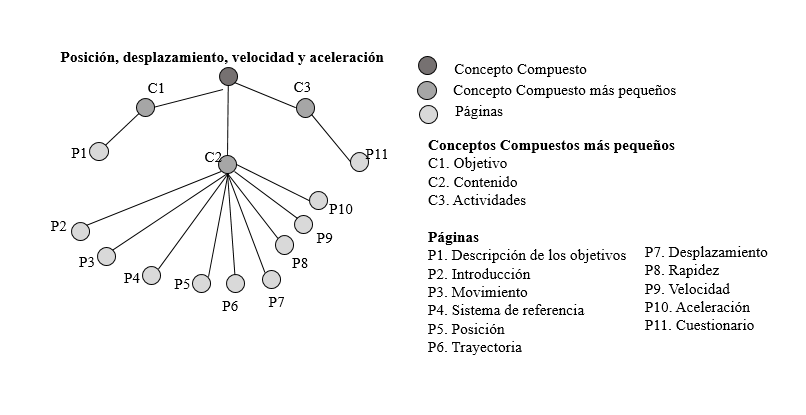
\includegraphics[scale=0.7]{Capitulo_4/2_XP/imagenes/unidad1.png}
    \caption{Estructura de la unidad 1:}
    \scriptsize \textbf{Fuente:} Elaboración propia
    \label{fig:estructura}
\end{figure}
\end{itemize}

Para el contenido en detalle de los modelos de dominio por cada unidad ver \textbf{(Carpeta Anexos, documento: Unidades de aprendizaje}.

\subsection{Fase II: Selección de teorías de estilos cognitivos}
Si se parte de la idea que “No todos los estudiantes piensan de la misma manera, ¿cómo pueden esperar que todos aprendan de la misma manera?” \cite{Graham2015}, de allí la importancia de prestarle atención a los estilos cognitivos de los estudiantes en su aprendizaje. 

Cuando un estudiante, diagnostica y usa su estilo cognitivo correctamente, hay un aumento significativo en el rendimiento académico \cite{Graham2015}.

Teniendo en cuenta lo anterior y los resultados obtenidos en la encuesta cognitiva I (véase tabla \ref{tab:EC}) realizada en la Institución Educativa Juan María Céspedes donde se refleja que los estudiantes poseen ciertas preferencias a la hora de estructurar los contenidos, con este proyecto no solo se buscó la creación de una aplicación que permitiera el aprendizaje de la materia Física en Décimo grado, sino que se buscó que la misma se adaptara a cada estudiante según los estilos cognitivos, permitiendo con ello que estos tuviesen la oportunidad de explorar los contenidos y conceptos según lo indica su estilo cognitivo. 

Ahora bien, la teoría de estilos cognitivos que se usó fue la teoría de Witkin donde clasifica los estilos cognitivos como independencia y dependencia del campo; ya que como lo indica  \cite{Ferraro2006}, es ``ampliamente validado y aplicado en numerosas investigaciones en el ámbito de sistemas hipermedia y sistema hipermedia adaptativa para el aprendizaje”.

\subsection{Fase III: Adaptación para el aprendizaje}
\textbf{Modelo del Estudiante:}\ \\
El instrumento que se utilizó para determinar los estilos cognitivos seleccionados se basó en el Test de Figuras enmascaradas, el cual consta de una prueba que evalúa los estilos cognitivos independiente y dependiente del campo, esta prueba se realiza a través de un folleto desarrollado por Witkin y su equipo, el cual se responde a lápiz por cada individuo. Durante la prueba las personas se hallan ante figuras visuales simples escondidas en figuras visuales complejas y se espera que ubiquen la forma o figura simple oculta en la más compleja en un tiempo determinado (véase Figura \ref{fig:papel}).

Se considera que las personas con estilo cognitivo dependientes del campo (DC) tienen más problemas para descubrir las formas simples ocultas, a diferencia de aquellos que poseen un estilo cognitivo independiente del campo (IC). Lo anterior debido a que las personas con DC tienen una percepción fuertemente dominada por el campo; por ejemplo, un estudiante en un bosque: si el estudiante posee un estilo cognitivo DC, solo verá el bosque como un todo; mientras que, si el estudiante posee un estilo cognitivo IC, este verá dentro del bosque, un árbol, pájaros, entre otros, es decir, verá por separado los elementos que componen dicho bosque. Por lo tanto, en esta prueba cuantas más figuras simples ocultas se encuentren, más independiente del campo será el sujeto, y cuantas menos figuras simples ocultas se encuentre, más dependiente del campo será el mismo.

Por otro lado, en la realización de este Test de Figuras enmascaradas, se requiere que todos los participantes estén en un el mismo lugar de prueba y, se requiere de un análisis de los resultados que puede llegar a ser tedioso y propenso a errores. Por ello para el presente proyecto se diseñó una versión digital (véase Figura \ref{fig:digital}) basada en el Online Group Embedded Figures Test, desarrollado por la Universidad de Gannon \cite{Yoo2006}. 

Cabe destacar que esta versión digital según \cite{Yoo2015} cumple con los mismos resultados que la versión en papel, con la característica fundamental de que los mismos se generan de manera instantánea una vez terminada la prueba.

\begin{figure}[H]
    \centering
    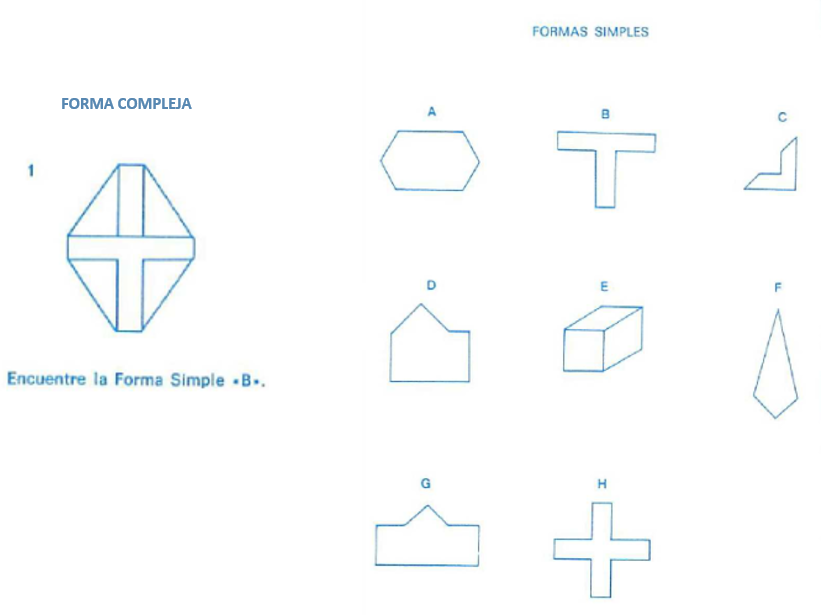
\includegraphics[scale=0.6]{Capitulo_4/2_XP/imagenes/papel.png}
    \caption{Test de Figuras enmascaradas en papel}
     \scriptsize \textbf{Fuente: }\cite{cuadernillo}
    \label{fig:papel}
\end{figure}

\begin{figure}[H]
    \centering
    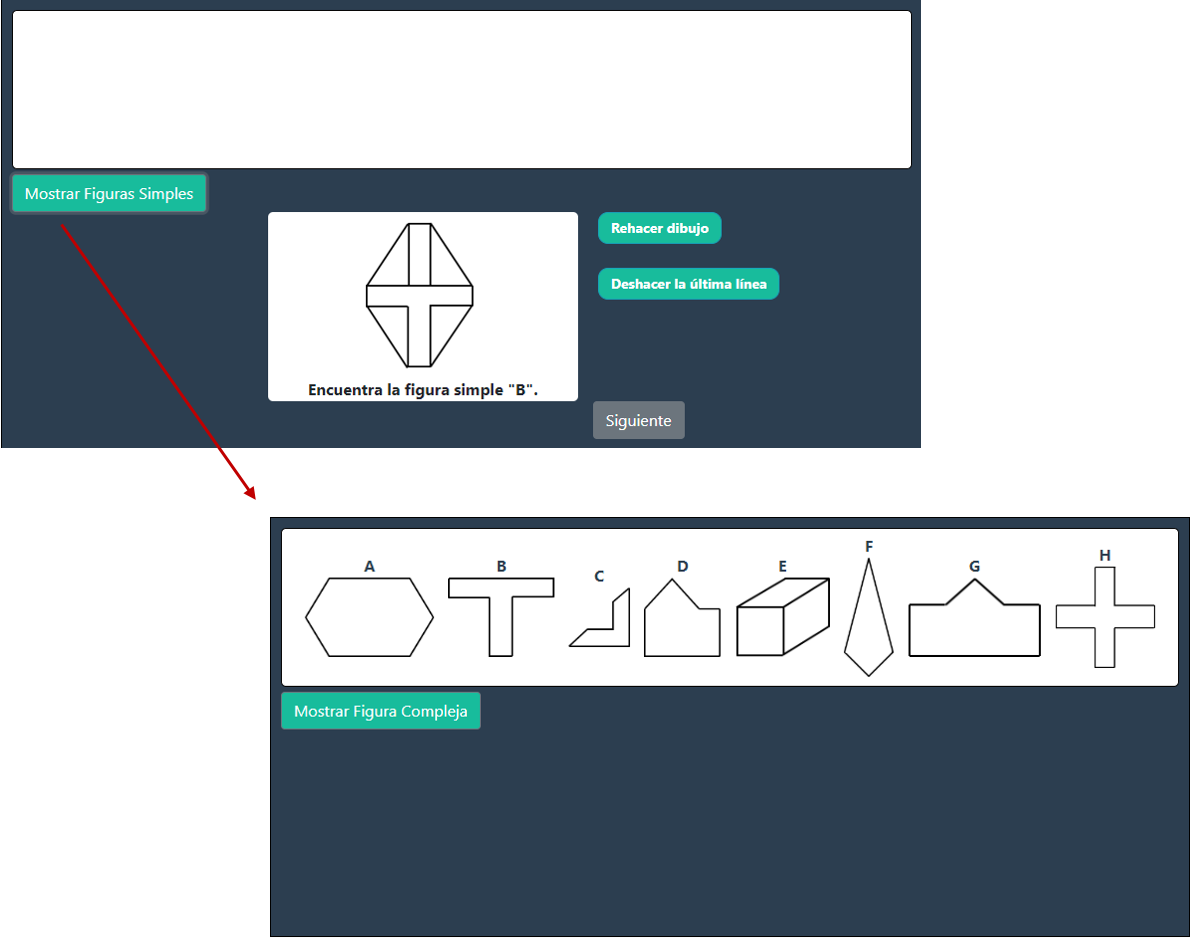
\includegraphics[scale=0.5]{Capitulo_4/2_XP/imagenes/virtual.png}
    \caption{Test de Figuras enmascaradas Digital}
     \scriptsize \textbf{Fuente: }Elaboración propia
    \label{fig:digital}
\end{figure}

\ \\ \textbf{Modelo de enseñanza}\ \\
Como ya se ha mencionado, los sistemas hipermedia adaptativo basados en estilos cognitivos, se adaptan especialmente las opciones de navegación. Para este caso, los estilos cognitivos elegidos son independiente del campo y dependiente del campo, en \cite{Ruttun2009} especifican, que los estudiantes con estilos cognitivos dependiente del campo cuando tienen que reestructurar nueva información tienen más probabilidades de enfrentar dificultades en un entorno no estructurado o no lineal, por ende, prefieren la guía de navegación o la representación en formato lineal del contenido. Mientras que, los estudiantes independientes del campo se sienten más cómodos con la presentación en formato no lineal. Se caracterizan por ser individuos que disfrutan trabajando solos y prefieren la navegación libre.

Por su parte, \cite{Dufresne1997} señala que los independientes del campo reorganizan activamente la información de acuerdo con las demandas contextuales e imponen una estructura cuando es necesario de acuerdo a su experiencia. Los dependientes del campo, por otro lado, siguen más fácilmente un enfoque estructurado y secuenciado, es decir, prefieren ser guiados.

En consecuencia, la aplicación hipermedia desarrollada buscó que se adaptara como muestra en la siguiente tabla:

\begin{table}[H]
    \centering
    \begin{tabular}{|p{5cm}|p{5cm}|}
        \hline
        \textbf{Estilo cognitivo} & \textbf{Recorrido de Navegación } \\
        \hline
        Independiente del Campo.&Libre \\
        \hline
         Dependiente del Campo.&Lineal\\
        \hline
    \end{tabular}
    \caption{Adaptación de la navegación de la aplicación}
    \centering \scriptsize \textbf{Fuente:} Elaboración propia
    \label{tab:adaptNav}
\end{table}


